%  Copyright 2020-2026 Robert Bosch GmbH
%
%  Licensed under the Apache License, Version 2.0 (the "License");
%  you may not use this file except in compliance with the License.
%  You may obtain a copy of the License at
%
%      http://www.apache.org/licenses/LICENSE-2.0
%
%  Unless required by applicable law or agreed to in writing, software
%  distributed under the License is distributed on an "AS IS" BASIS,
%  WITHOUT WARRANTIES OR CONDITIONS OF ANY KIND, either express or implied.
%  See the License for the specific language governing permissions and
%  limitations under the License.

\newpage
\section{Configuration}
Before using GitHub Copilot, you need to sign in with your GitHub account
and enable the extension.
To do this, follow these steps:
\begin{itemize}
   \item Click on the \textbf{GitHub Copilot} icon in the Activity Bar.
   \item Then Click on the \textbf{Sign in} button of
         \textbf{GitHub Copilot Cloud Agent} section as below:

\begin{boxhint}{Warning}
The \textbf{Sign in} button of \textbf{GitHub Copilot Cloud Agent} may not be visible
in some cases due to limited vertical space, as the \textbf{GitHub Copilot CLI Agent} may overlap
and hide the \textbf{Sign in} button.

In this case, scroll down within the \textbf{GitHub Copilot Cloud Agent} panel or resize the panel
to reveal the \textbf{Sign in} button.
\end{boxhint}

         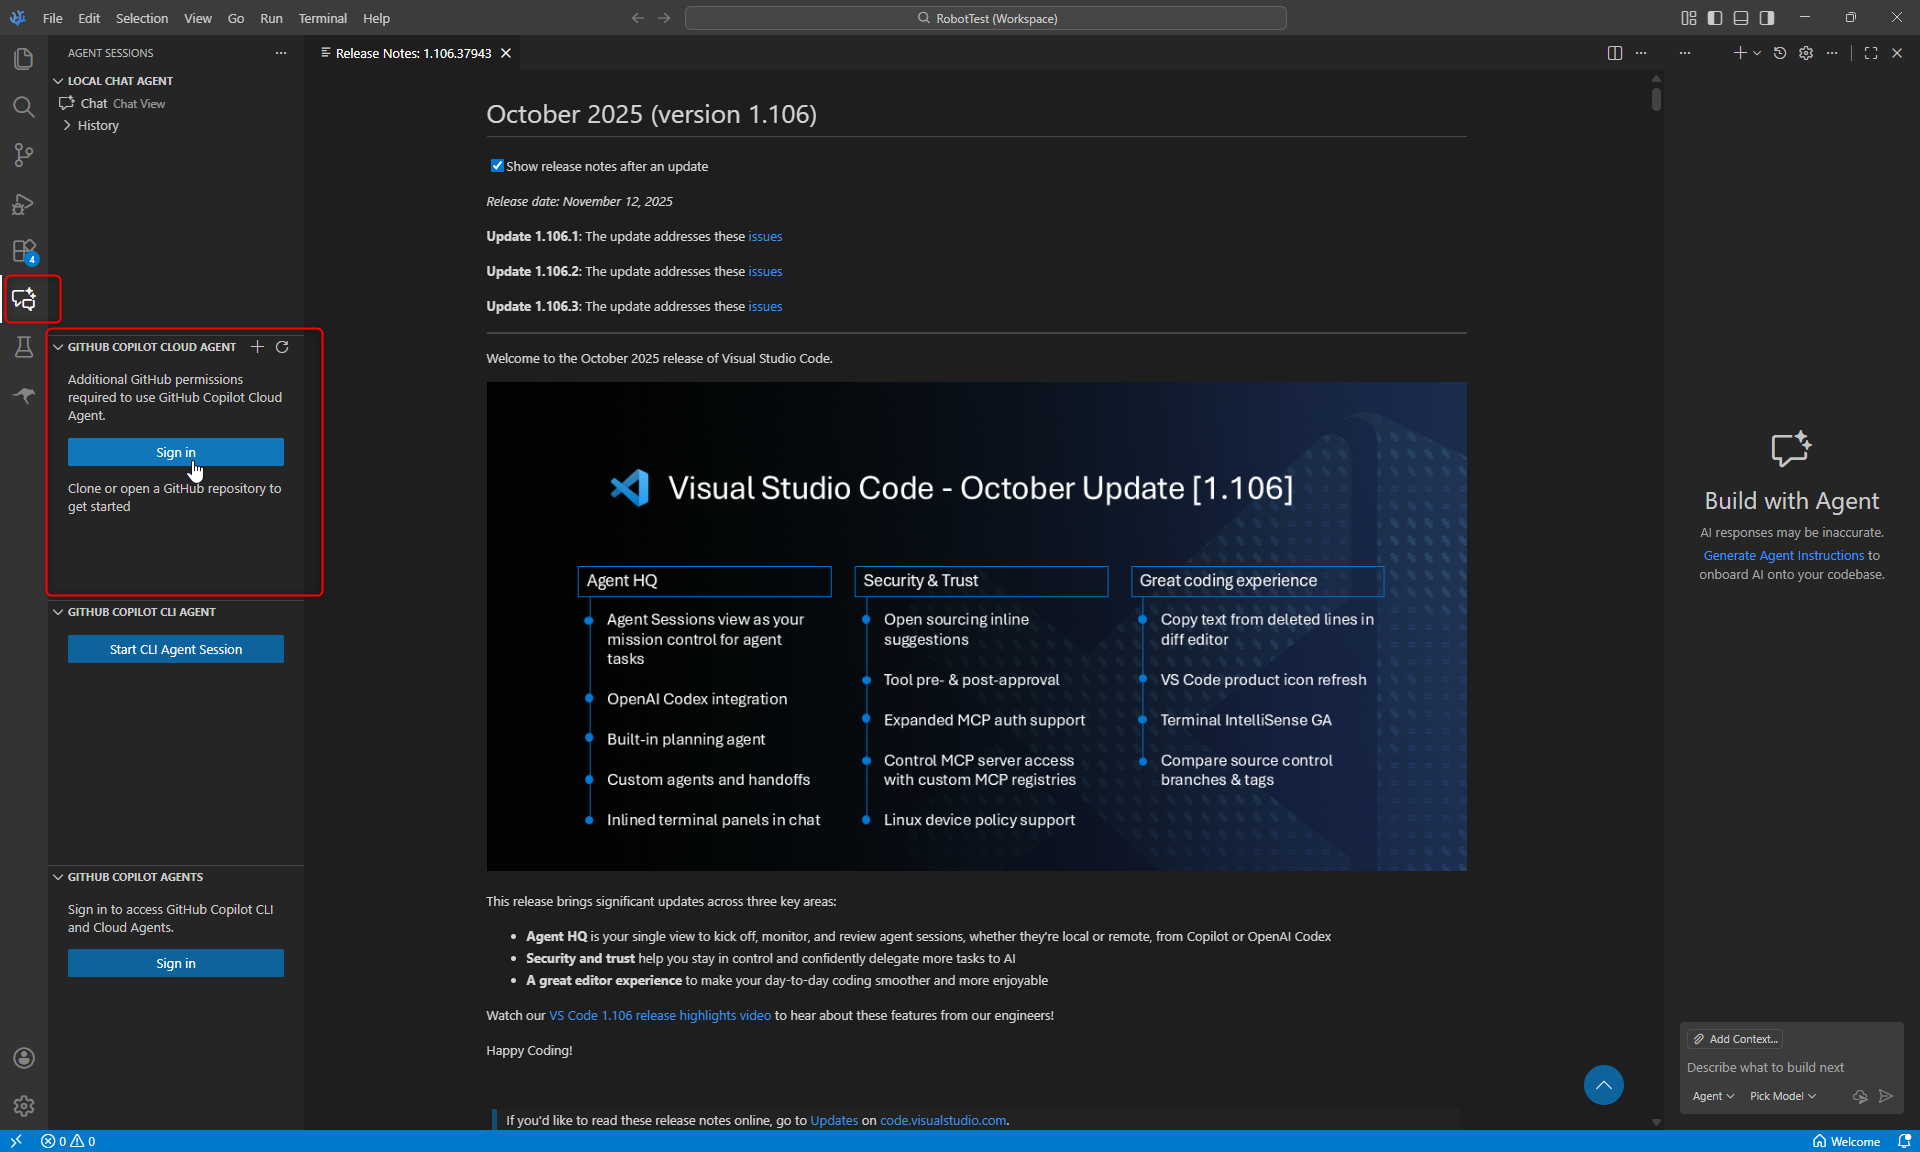
\includegraphics[width=0.9\textwidth]{./include/graphics/copilot/configuration_step_1_signin.png}

   \item The pop-up will appear to ask the permission for
         \textbf{GitHub Copilot Chat} extension.

         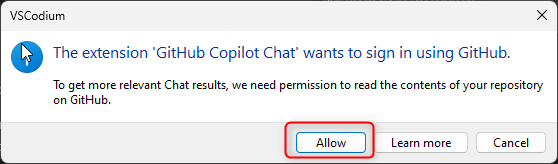
\includegraphics[width=0.5\textwidth]{./include/graphics/copilot/configuration_step_2_allow.png}

         Click \textbf{Allow} to move to next step.

\begin{boxhint}{Warning}
If the below pop-up appears instead:

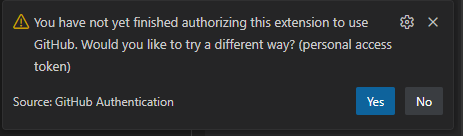
\includegraphics[width=0.5\textwidth]{./include/graphics/copilot/internet_access_issue.png}

It may indicate that the internet access is not available for GitHub Copilot extension,
please check your network connection and proxy settings if applicable.

Details about how to configure proxy for \textbf{VsCodium For RobotFramework} can be found
\hyperref[fw-environment-environment-proxy-configuration]{here}.
\end{boxhint}

   \item The authentication code will be displayed in the pop-up window as below:

         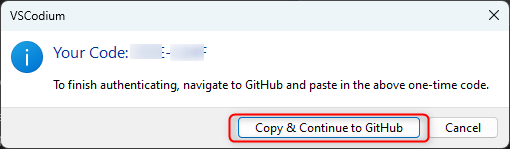
\includegraphics[width=0.5\textwidth]{./include/graphics/copilot/configuration_step_3_auth_code.png}

         Click \textbf{Copy \& Continue to Github} button
         then click \textbf{Open} the GitHub sign-in page in your web browser.

         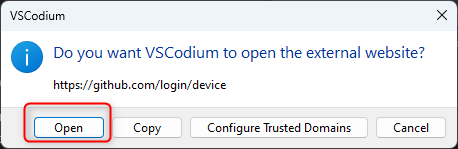
\includegraphics[width=0.5\textwidth]{./include/graphics/copilot/configuration_step_4_open_browser.png}

   \item In the GitHub sign-in page, paste the authentication code and click \textbf{Continue} button.
   \item Then, the last confirmation page will appear as below:

         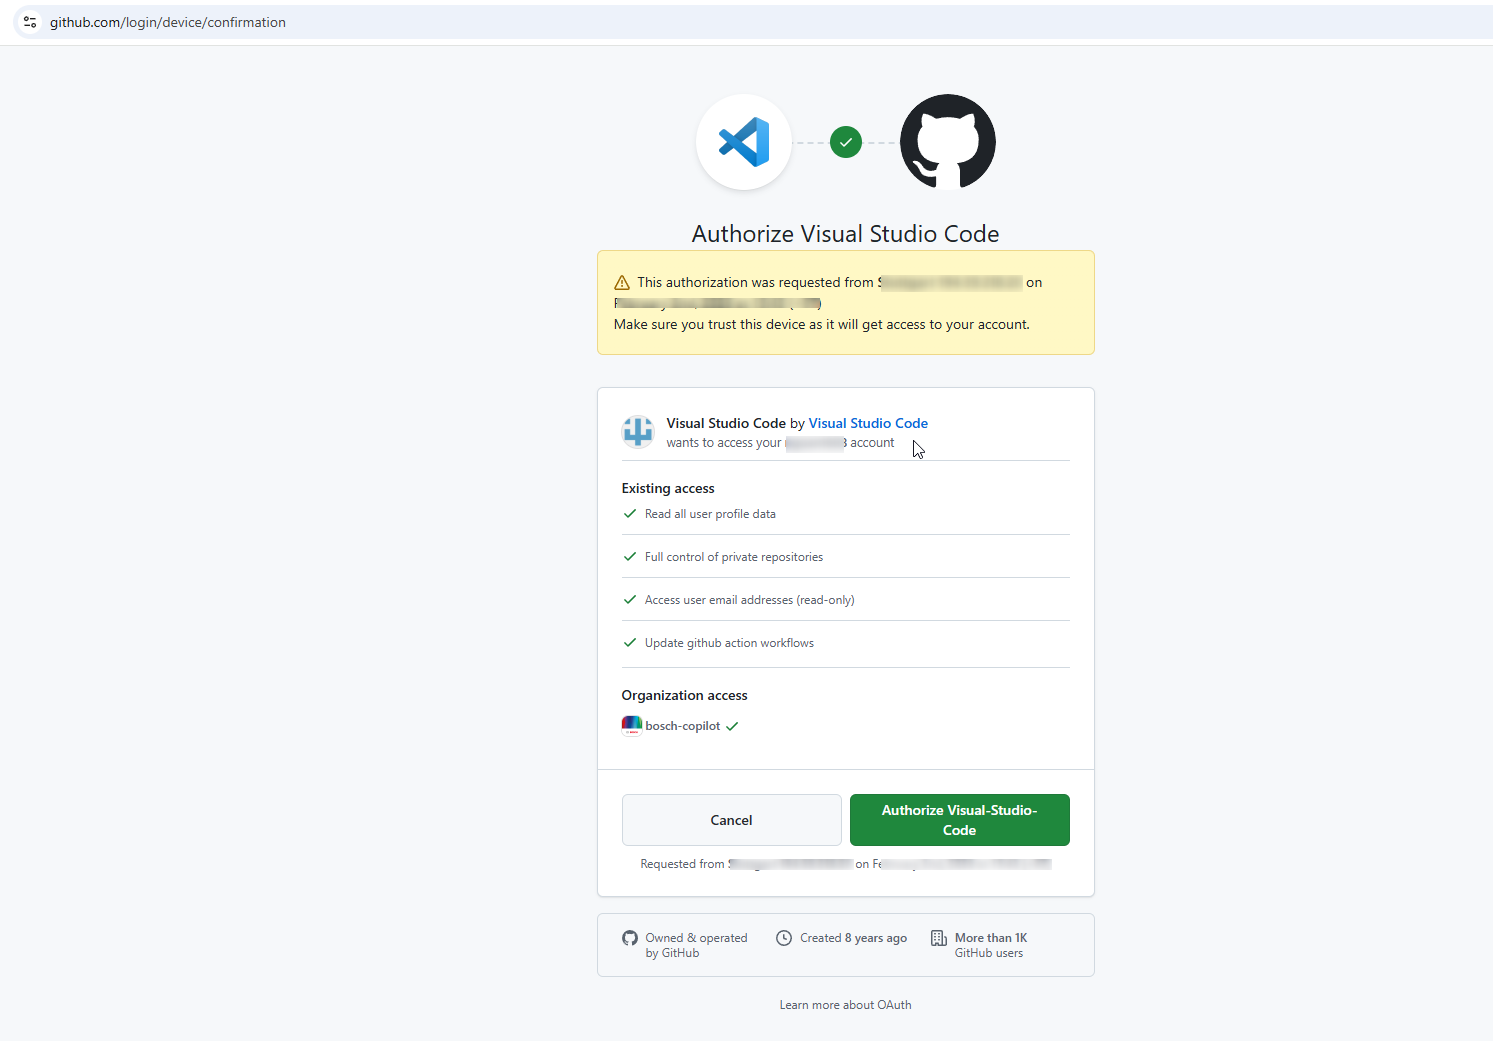
\includegraphics[width=0.9\textwidth]{./include/graphics/copilot/configuration_step_5_confirm.png}

         Click \textbf{Authorize Visual Studio Code} button to complete the sign-in process.
   \item Now back to \textbf{VSCodium For RobotFramework}, the GitHub Copilot extension is enabled and ready to use.
\end{itemize}

With GitHub Copilot enabled, you can enhance your coding experience
and boost your productivity in \textbf{VSCodium For RobotFramework}.
